\documentclass[a4paper,english]{article}
\usepackage{graphicx}
\usepackage{listings}
%% Use utf-8 encoding for foreign characters
%%\usepackage[T1]{fontenc}
%%\usepackage[utf8]{inputenc}
%%\usepackage{babel}
%%
%%%% Vector based fonts instead of bitmaps
%%\usepackage{lmodern}
%%
%%%% Useful
%%%\usepackage{fullpage} % Smaller margins
%%\usepackage{enumerate}
%%
%%%% Theorem
%%\usepackage{amsthm}
%%
%%%% More math
%%\usepackage{amsmath}
%%\usepackage{amssymb}
\lstset{
  breaklines=true,
  postbreak=\mbox{{$\hookrightarrow$}\space},
}
%% Document Header
\title{Section5}
\author{Elliott Ashby}
\date{\today}

\begin{document}
    \maketitle
    \section{q1}
        The code first makes a list of 10 zeros then generates random numbers between 1 and 10 and increments the respective index of the list by 1. Therefore what is printed is
        a count of how many times each number is generated.
        \\
    \section{q2}
        We generate 1000 random numbers in order to minimise the random aspect of the code, the more random numbers are generated the more obvious the actual pattern appears to be.
        \\
    \section{q3}
    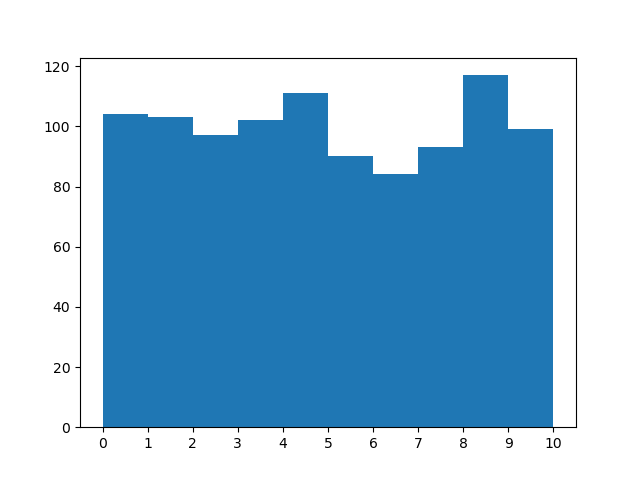
\includegraphics[scale=0.8]{q5_3.png}
    \\
    \section{q4}
        \lstinputlisting[language=Python, firstline=12, lastline=18]{./q5_1.py}
        \lstinputlisting[language=Python]{./q5_4.py}
        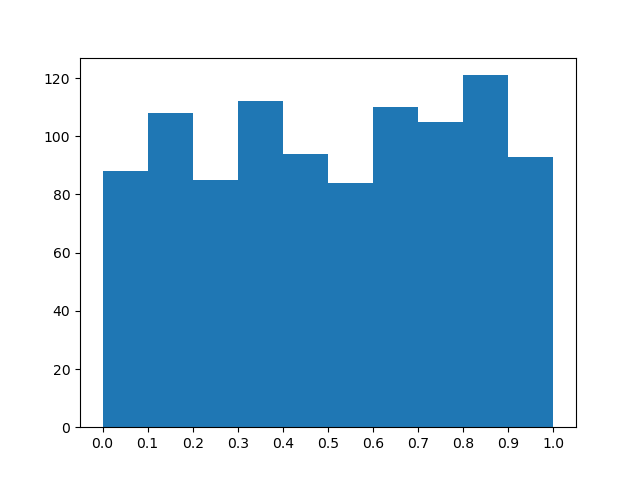
\includegraphics[scale=0.8]{q5_4.png}
        \\
    \section{q5}
        \lstinputlisting[language=Python, firstline=12, lastline=18]{./q5_1.py}
        \lstinputlisting[language=Python]{./q5_5.py}
        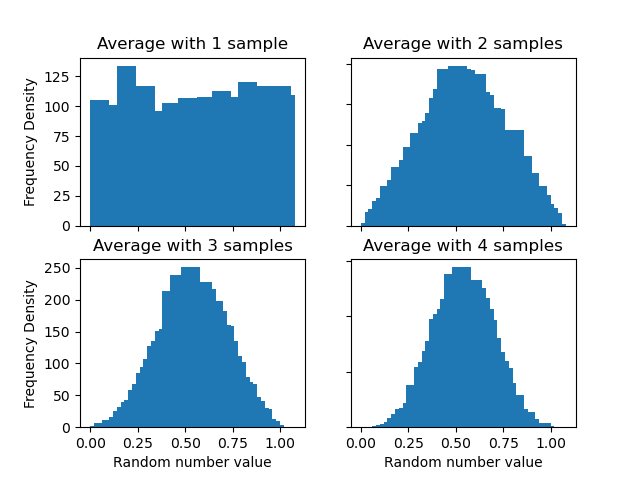
\includegraphics[scale=0.8]{q5_5.png}
        \\
    \section{q6}
        Averages of random numbers converge at the center most value, this makes sense since if there are an equal number of 
        numbers accross the whole range, their average is the center most value.
        \\
    \section{q7}
        \lstinputlisting[language=Python, firstline=21, lastline=26]{./q5_1.py}
        \lstinputlisting[language=Python]{./q5_7.py}
        Simply count how many of the randomly generated numbers fall in the range and find that as a fraction of the total numbers
        generated. This is the percentage of numbers within the range, all numbers outside of that range is the opposite value, so 1 - that value
        gives you the percentage of randomly generated numebers outside of the range.
        \\
    \section{q8}
        \lstinputlisting[language=Python]{./q5_8.py}
        This results in an output of around:
        $15\pm0.01$,
        Which confirms that the poisson data set of mean 15 actually has a mean of 15.
        \\
    \section{q9}
        \lstinputlisting[language=Python]{./q5_9.py}
        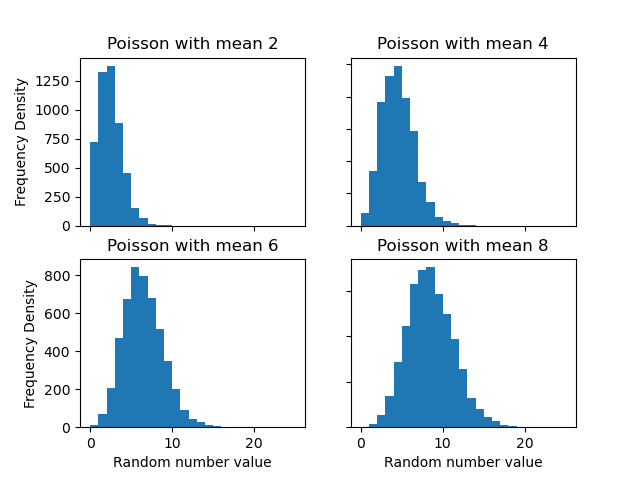
\includegraphics[scale=0.8]{q5_9.png}
        \\
    \section{q10}
        As the mean increases, the histogram shifts to the right as the mean becomes the value with the largest count, in addition
        the poisson width increases. A poisson with a low mean is skewed with a tail only extending to the right. As the mean increases 
        the distribution spreads out to become more symmetric. This is because in a poisson distribution, the mean is equal to the 
        variance.
\end{document}
